% ltex: language=it
\chapter{Deep Learning}\label{chap:deep_learning} % (fold)
\section{Introduzione}\label{sec:dl_introduzione} % (fold)
Con il termine \ac{dnn} si denotano reti <<profonde>> composte da molti livelli organizzati gerarchicamente.
\\
Le implicazioni di universal approximation theroem e la difficoltà di addestrare reti con livelli hanno portato per lungo tempo a focalizzarsi su reti con un solo livello hidden.
L'esistenza di soluzioni non implica efficienza: esistono funzioni computabili con complessità polinomiale operando su $k$ livelli, che richiedono una complessità esponenziale se si opera su $k-1$ livelli.
\emptyln{}
L'organizzazione gerarchica consente di \textbf{condividere} e \textbf{riusare} informazioni.
Lungo la gerarchia è possibile selezionare feature specifiche e scartare dettagli inutili al fine di massimizzare l'invarianza.
\begin{cimage}
    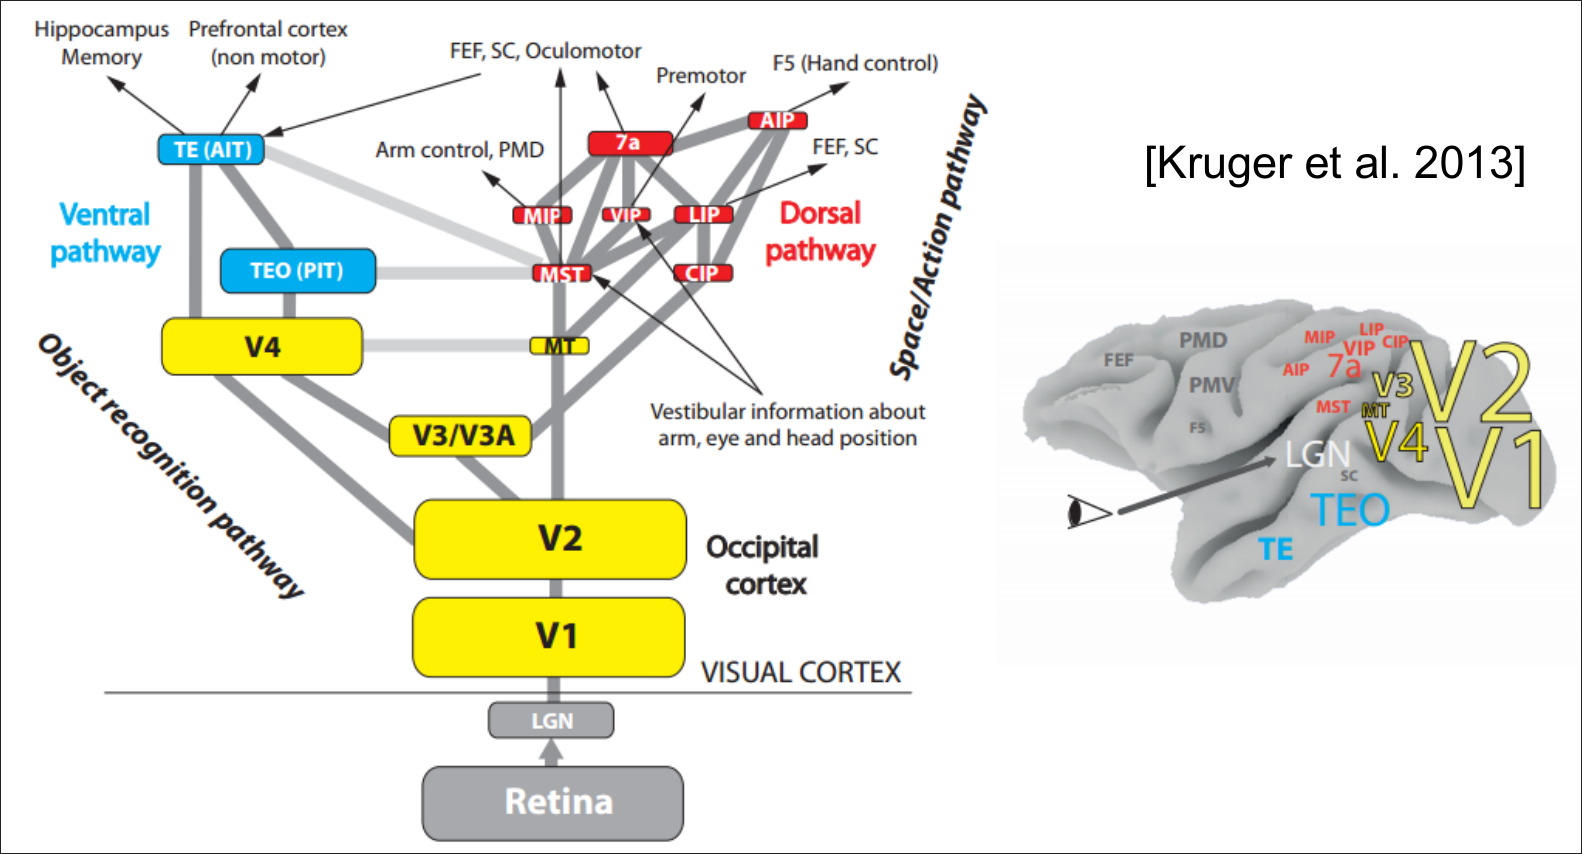
\includegraphics[width=.8\textwidth]{assets/why-deep-visual.png}
\end{cimage}
\begin{note}[Ma quanto deep?]
    Le \ac{dnn} oggi maggiormente utilizzate consistono di un numero di livelli compreso tra $7$ e $100$.
    Reti più profonde hanno dimostrato di poter garantire prestazioni leggermente miglior, a discapito dell'efficienza.
\end{note}
\subsection{Livelli e Complessità}\label{sub:livelli_e_complessita} % (fold)
La profondità (numero di livelli) è solo uno dei fattori di complessità.
Il numero di \textbf{neuroni}, di \textbf{connessioni} e di \textbf{pesi} caratterizzano altresì la complessità di una \ac{dnn}.
\\
Maggiore è il numero di \red{pesi}, ovvero di \red{parametri da apprendere}, maggiore è la complessità del \textbf{training}.
Al tempo stesso un elevato numero di \red{neuroni} e \red{connessioni} rende \textbf{forward} e \textbf{back propagation} più costosi, poiché aumenta il numero di operazioni necessarie.
\begin{cimage}
    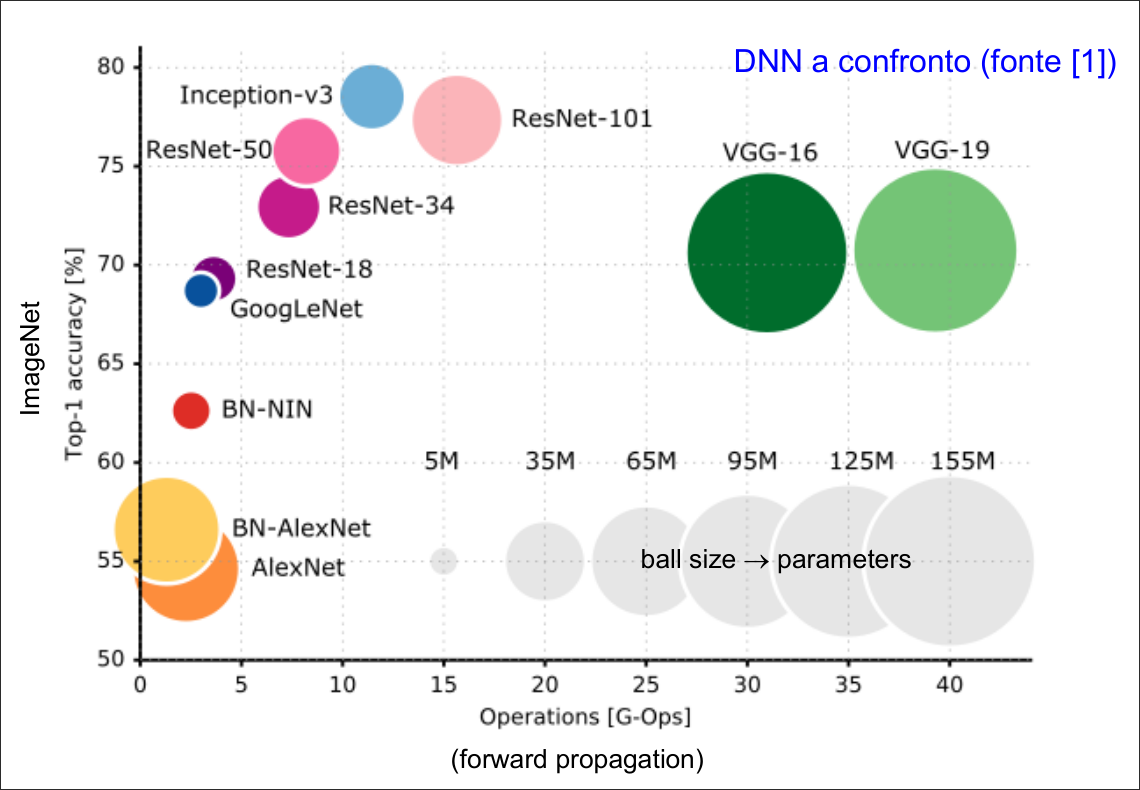
\includegraphics[width=.8\textwidth]{assets/dnn-comparison-visual.png}
\end{cimage}
% subsection Livelli e complessita (end)
%
\subsection{Tipologie di DNN}\label{sub:tipologie_di_dnn} % (fold)
\begin{itemize}
    \item[] Modelli feedforward <<\textbf{discriminativi}>> per la classificazione, o regressione, con training prevalentemente \red{supervisionato}:
        \begin{itemize}
            \item \ac{fcdnn} (MLP con almeno due livelli hidden);
            \item \ac{cnn} (o ConvNet);
        \end{itemize}
    \item[] Modelli ricorrenti con \textbf{memoria e attenzione}:
        \begin{itemize}
            \item \ac{rnn};
            \item \ac{lstm};
            \item \red{Transformers};
        \end{itemize}
    \item[] Addestramento \red{non supervisionato} (modelli addestrati a ricostruire l'input e utilizzati per denoising, anomaly detection, ...):
        \begin{itemize}
            \item \ac{gan};
            \item \ac{vae};
        \end{itemize}
    \item[] Reinforcement learning, per apprendere comportamenti:
        \begin{itemize}
            \item Deep Q-Learning;
        \end{itemize}
\end{itemize}
\newpage
\begin{description}
    \item[Big Data]: disponibilità di dataset etichettati di grandi dimensioni.
        \\
        La superiorità delle tecniche di deep learning rispetto ad altri approcci si manifesta quando sono disponibili \red{grandi quantità} di dati di training.
        \begin{cimage}
            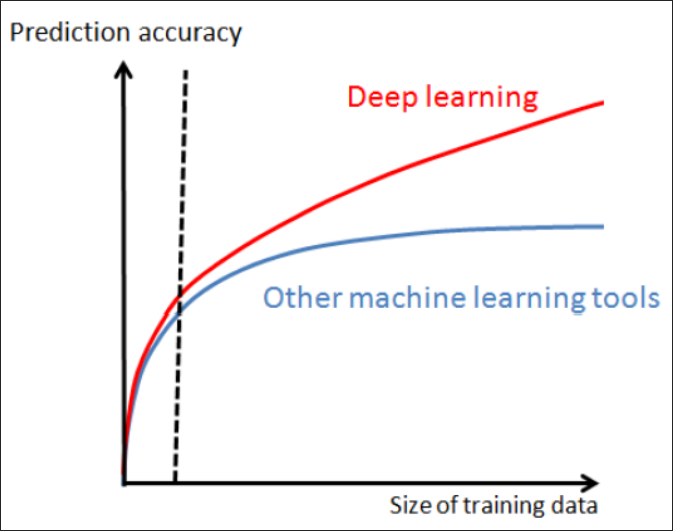
\includegraphics[width=.4\textwidth]{assets/big-data-visual.png}
        \end{cimage}
    
    \item[GPU Computing]: il training di modelli complessi, profondi e con molti pesi e connessioni, richiede elevate potenze computazionali.
        La disponibilità di GPU con migliaia di core e GB di memoria interna ha consentito di ridurre drasticamente i tempi di training.
    \item[Vanishing gradient]\label{it:vani-grad}: la retro propagazione del gradiente è problematica su reti profonde se si utilizza la \hyperref[par:sigmoid]{sigmoide} come funzione di attivazione.
        Il problema può essere gestito con attivazione \textbf{Relu} e migliore \hyperref[sub:inizializzazione_dei_pesi]{inizializzazione dei pesi}.
\end{description}
% subsection Tipologie di DNN (end)
%
\subsection{Funzione di attivazione: Relu}\label{sub:funzione_di_attivazione_relu} % (fold)
Nelle reti \ac{mlp} la funzione di attivazione più utilizzata è la \hyperref[par:sigmoid]{sigmoide}.
Nelle reti profonde, l'utilizzo della sigmoide è problematico per la retro propagazione del gradiente (problema del \textbf{vanishing gradient}: la derivata della sigmoide è tipicamente minore di 1 e l'applicazione della regola di derivazione a catena porta a moltiplicare molti termini minori di 1 con la conseguenza di ridurre parecchio i valori del gradiente nei livelli lontani dall'output.
\\
La sigmoide ha un comportamento \red{saturante}, allontanandosi dallo 0.
Nelle regioni di saturazione la derivata vale 0 e pertanto il gradiente si annulla.
\emptyln{}
L'utilizzo di \ac{relu} come funzione di attivazione risolve il problema:
\[
    \fx[net] = \max{\pt{0,\,net}}
\]
\begin{cimage}
    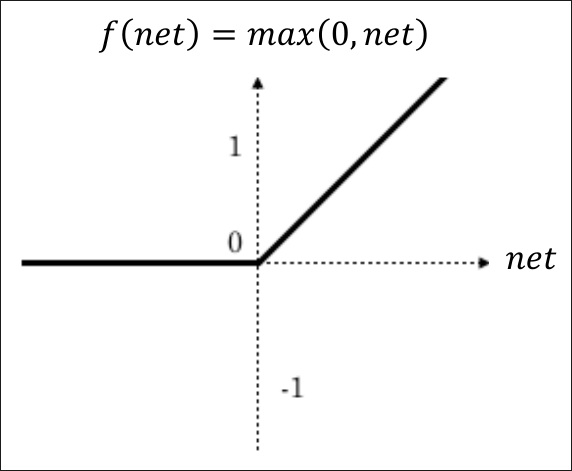
\includegraphics[width=.6\textwidth]{assets/relu-func-visual.png}
\end{cimage}
\begin{itemize}
    \item la derivata vale $0$ per valori negativi o nulli di $net$ e $1$ per valori positivi;
    \item per valori positivi nessuna saturazione;
    \item porta ad attivazioni \red{sparse} (parte dei neuroni sono spenti) conferendo maggiore robustezza alla rete;
\end{itemize}
\subsubsection{Varianti}\label{sec:relu_varianti} % (fold)
Sebbene \ac{relu} sia spesso la funzione di attivazione di default, alcune delle sue varianti possono essere più efficaci.
\begin{itemize}
    \item \textbf{Leaky Relu}, evita che nella parte negativa il gradiente sia 0, e quindi permette ai neuroni spenti durante il training di potersi attivare;
    \item \ac{elu} oltre a non avere gradiente nullo nella parte negativa, è più smoothed vicino allo 0 (no discontinuità per $\al = 1$);
\end{itemize}
\begin{cimage}
    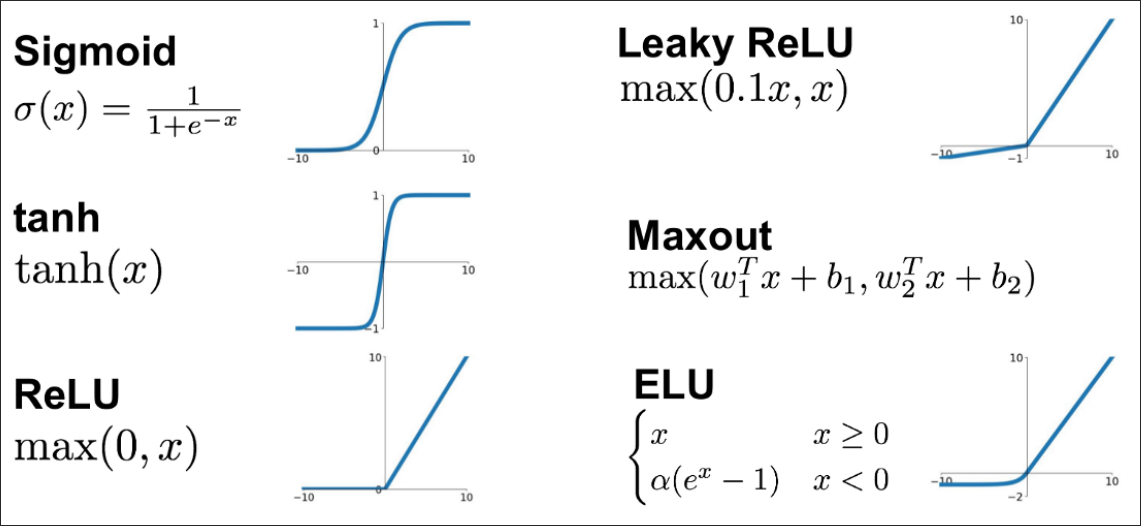
\includegraphics[width=.8\textwidth]{assets/active-func-visual.png}
\end{cimage}
% subsubsection Relu: varianti (end)
% subsection Funzione di attivazione: Relu (end)
%
\subsection{Dropout}\label{sub:dropout} % (fold)
È una tecnica di regolarizzazione utile per controllare l'overfitting:
\begin{itemize}
    \item specialmente nel caso di modelli molto grandi addestrati su dataset relativamente piccoli;
    \item rallenta la convergenza, ma può migliorare la generalizzazione;
    \item usato per addestrare AlexNet su ImageNet;
\end{itemize}
Durante il training alcuni neuroni spenti per far sì che l'output non dipenda da specifici neuroni, ma sia determinato in modo più robusto.
In \red{inference} tutti i neuroni sono attivi.
\begin{cimage}
    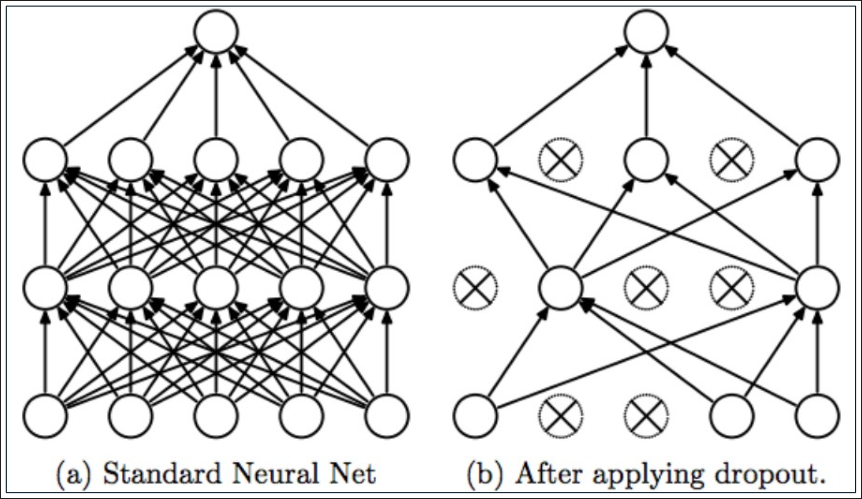
\includegraphics[width=.8\textwidth]{assets/dropout-visual.png}
\end{cimage}
\begin{note}
    In una \ac{cnn} è solitamente applicato solo ai livelli \red{fully connected} nella parte finale della rete, ma non all'output.
\end{note}
% subsection Dropout (end)
%
\subsection{Autodiff}\label{sub:autodiff} % (fold)
La maggior parte dei framework di deep learning rende disponibili meccanismi di composizione e propagazione automatica del gradiente attraverso \red{reverse-mode autodiff}:
\begin{itemize}
    \item si sfrutta la regola di derivazione a catena che permette di isolare il contributo di ogni layer (operatore) per poi ricomporre automaticamente i pezzi;
    \item se si definisce un nuovo layer $f$ non esistente per un framework è richiesto di definire solo i \textbf{gradienti locali}:
        \begin{itemize}
            \item $\dfrac{\dr y}{\dr x}$ dell'output $y$ rispetto all'input $x$;
            \item $\dfrac{\dr y}{\dr w}$ dell'output $y$ rispetto ai parametri locali $w$;
        \end{itemize}
\end{itemize}
\begin{note}
    La propagazione e combinazione con il resto dei gradienti è eseguita automaticamente
\end{note}
\begin{cimage}
    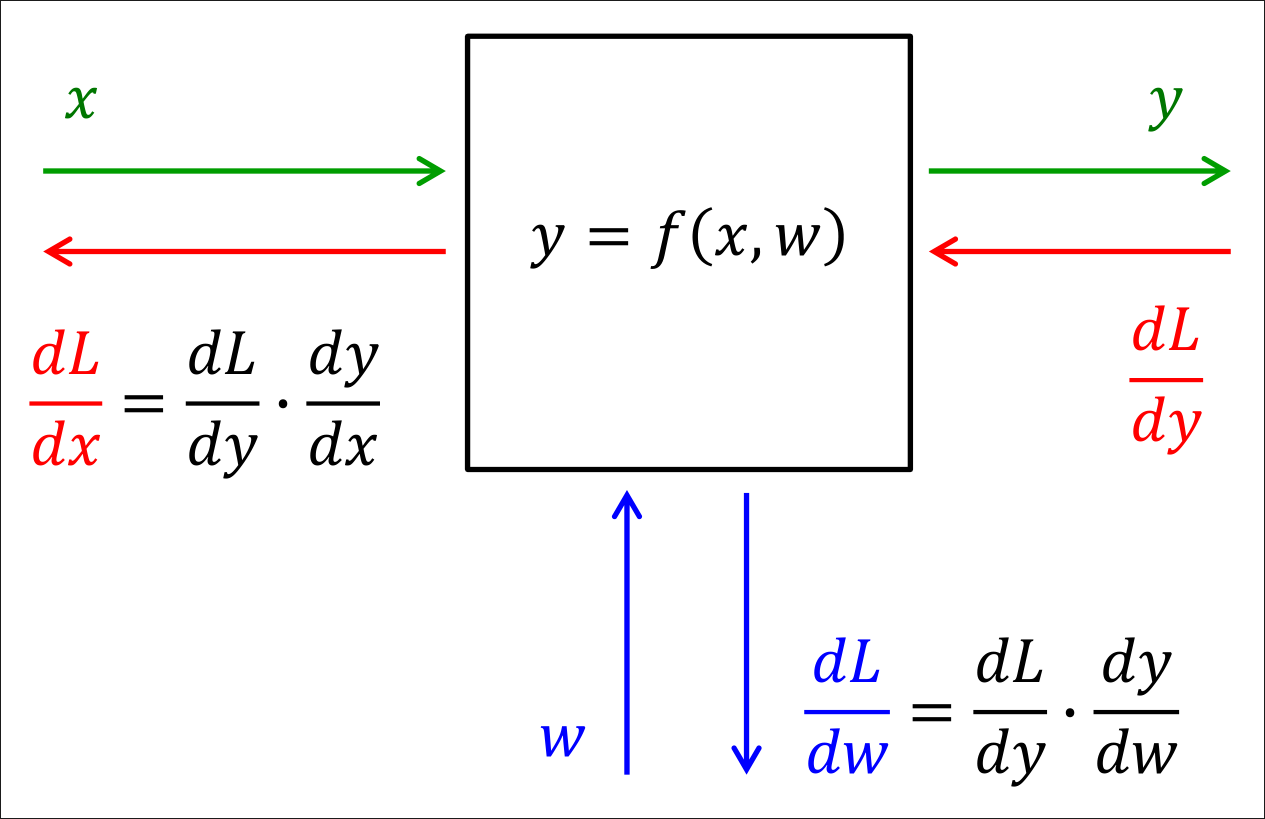
\includegraphics[width=.6\textwidth]{assets/autodiff-visual.png}
\end{cimage}
In pratica input, output e pesi di un livello sono organizzati in tensori (multidimensionali) e il calcolo dei gradienti richiede derivate parziali, organizzate in matrici \textbf{Jacobiane}.
\begin{quote}
    La chain rule può essere applicata \textbf{moltiplicando} tra loro matrici Jacobiane, con le necessarie trasposizioni.
    \\
    Le GPU risultano particolarmente adatte a eseguire moltiplicazioni \ac{gemm}.
\end{quote}
\begin{example}{Livello \red{fully connected} senza bias: $y = Wx$}{}
    \begin{cimage}
        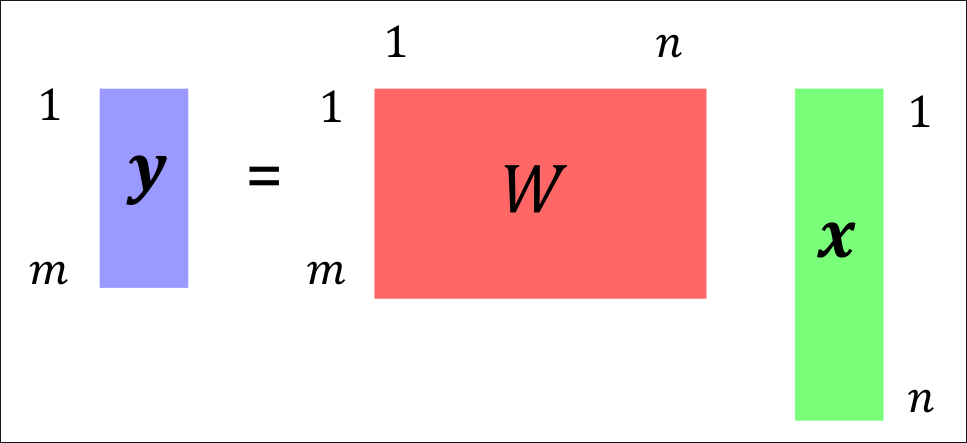
\includegraphics[width=.6\textwidth]{assets/autodiff-full-conn-ex.png}
    \end{cimage}
    \begin{itemize}
        \item $x \in \R[n]$ ($n$ neuroni di input);
        \item $y \in \R[m]$ ($m$ neuroni di output);
        \item $W \in \R[m\times n]$ (matrice dei pesi locali);
    \end{itemize}
    \[
        \frac{\dr y}{\dr x} = \ps{\frac{\dr y_i}{\dr x_j}} = \ps{W_{ij}} = W
    \]
    \[
        \frac{\dr y}{\dr W_i} = x, \qquad \for[][][m]
    \]
\end{example}
% subsection Autodiff (end)
% section Introduzione (end)
%
\section{Convolutional Neural Network}\label{sec:cnn} % (fold)
Le \ac{cnn} sono state progettate per processare \red{immagini}, per le quali l'elaborazione \textbf{locale}, pesi \textbf{condivisi} e \textbf{pooling} non solo semplificano il modello, ma lo rendono più efficace rispetto a modelli fully connected.
Possono essere utilizzate anche per altri tipi di pattern.
%
\subsection{Architettura}\label{sub:cnn_architettura} % (fold)
Una \ac{cnn} è composta da una gerarchia di livelli.
Il livello di \red{input} è direttamente collegato ai \textbf{pixel} dell'immagine, mentre gli \red{ultimi livelli} sono generalmente \textbf{fully-connected} e operano come un \hyperref[sec:mlp]{classificatore MLP}.
Nei livelli \red{intermedi} si utilizzano connessioni locali e pesi condivisi.
\begin{cimage}
    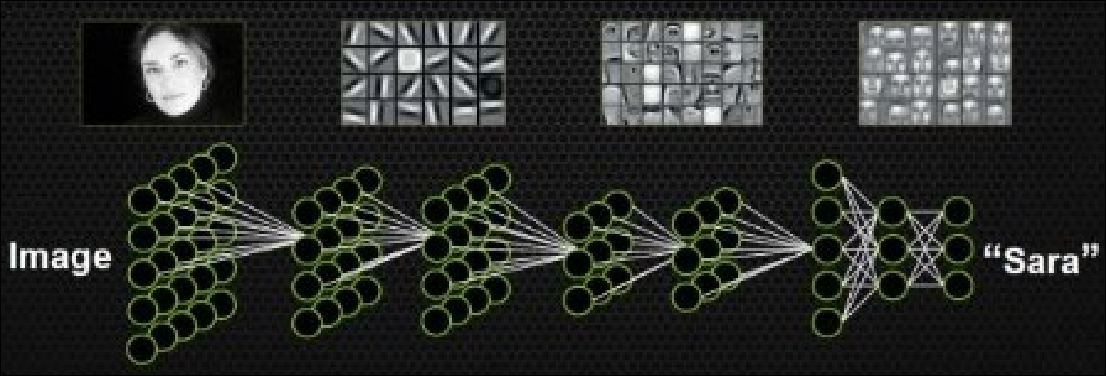
\includegraphics[width=.6\textwidth]{assets/cnn-arch-visual.png}
\end{cimage}
\begin{note}
    Il campo visivo dei neuroni, chiamato \textbf{receptive field}, aumenta muovendosi verso l'alto della gerarchia
\end{note}
Le connessioni \red{locali} fanno sì che i neuroni \textbf{processino nello stesso modo} porzioni diverse dell'immagine.
Si tratta di un comportamento desiderato, in quanto regioni diverse del campo visino contengono lo stesso tipo di informazioni (bordi, spigoli, porzioni di oggetti, ecc.).
% subsection Architettura (end)
%
\subsection{Convoluzione}\label{sub:cnn_convoluzione} % (fold)
La \textbf{convoluzione} è una delle più importanti operazioni di \textbf{image processing} attraverso la quale si applicano filtri digitali.
Un \textbf{filtro} digitale (maschera 2D di pesi) è fatto scorrere sulle diverse posizioni di input; per ogni posizione viene generato un valore di output, eseguendo il \textbf{prodotto scalare} tra la maschera e la porzione dell'input coperta.
\begin{cimage}
    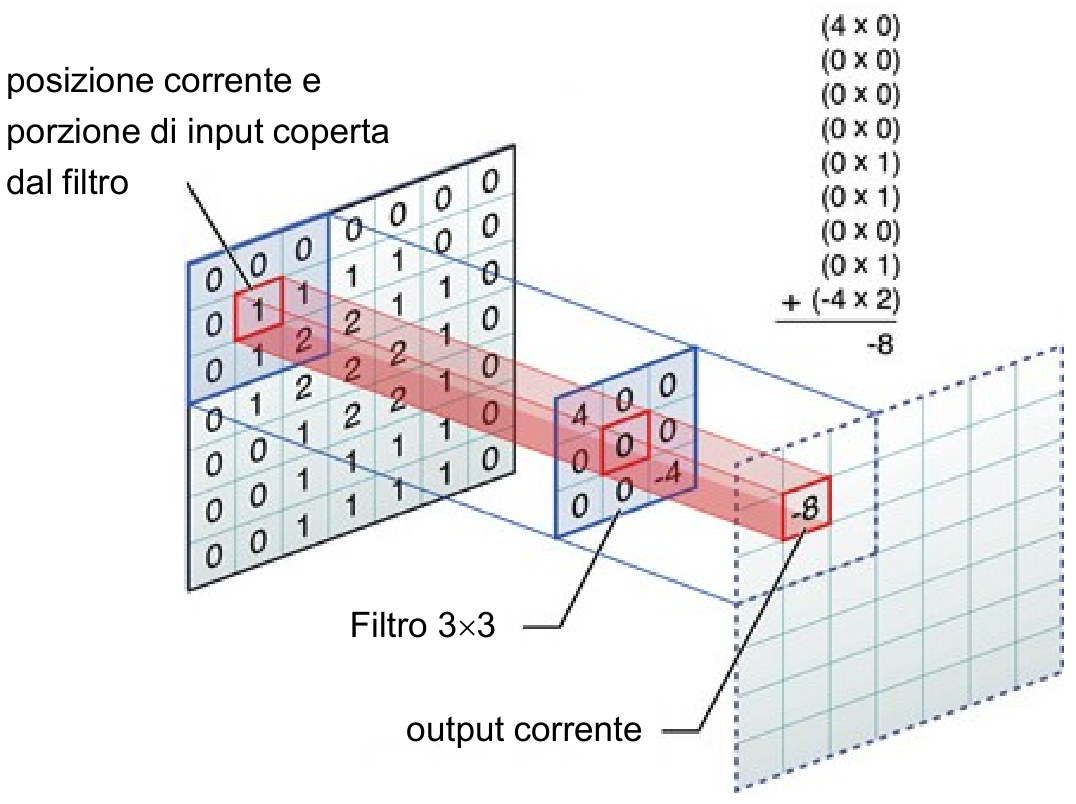
\includegraphics[width=.6\textwidth]{assets/convoluzione-visual.png}
\end{cimage}
\begin{description}
    \item[Neuroni come convolutori] Si considerano i pixel come neuroni e le due immagini di input e di output come livelli successivi di una rete.
        Dato un filtro $3\times 3$, se colleghiamo un neurone ai $9$ neuroni che esso <<copre>> nel livello precedente, e utilizziamo i pesi del filtro come pesi delle connessioni $w$, notiamo che un classico \textbf{neurone} di una \hyperref[sec:mlp]{MLP} esegue di fatto una \hyperref[sub:cnn_convoluzione]{convoluzione}.
        \begin{cimage}
            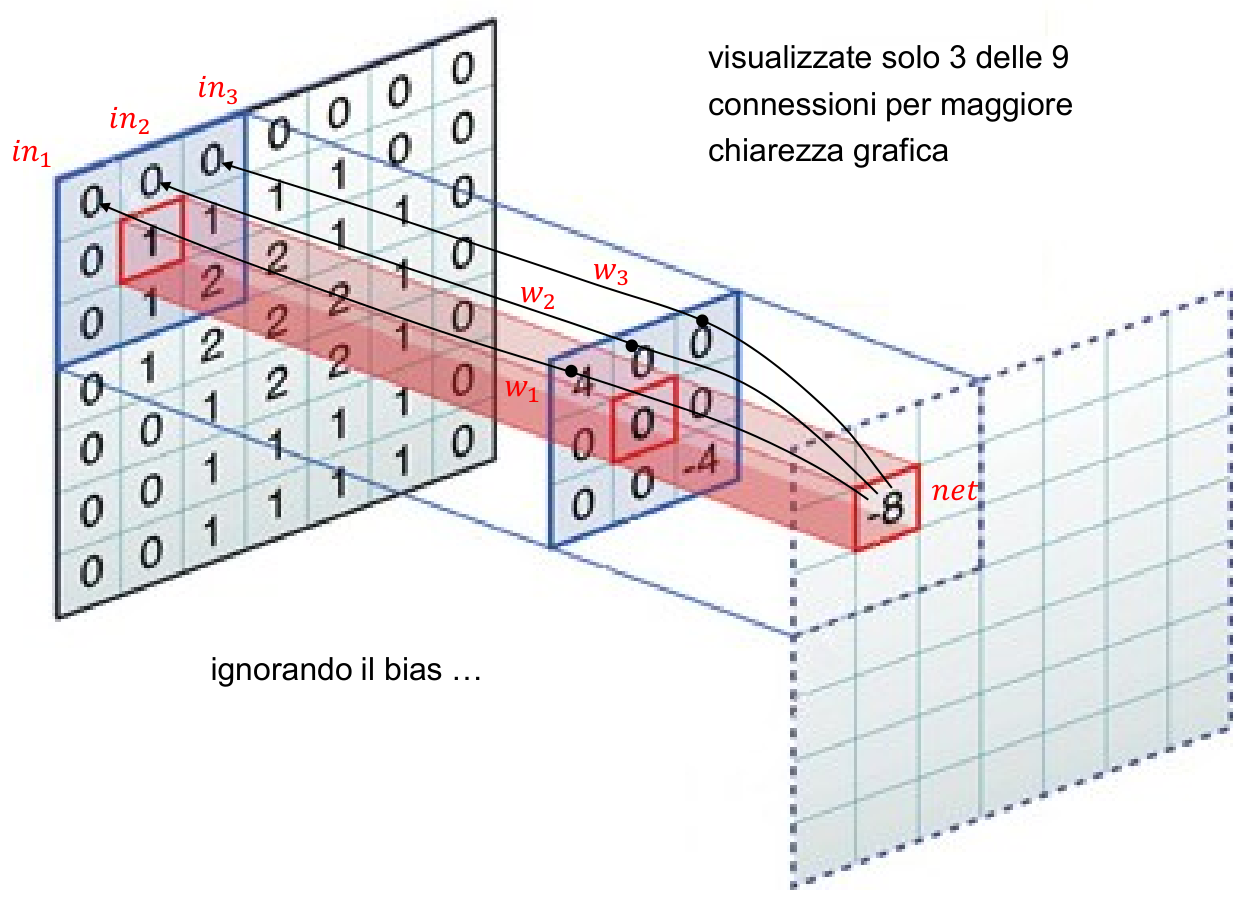
\includegraphics[width=.6\textwidth]{assets/neuro-conv-filter-visual.png}
        \end{cimage}
        \[
            net = \sum_{\for[j][][9]}{w_j\cdot in_j}
        \]
\end{description}
%
\subsubsection{Volumi}\label{sub:cnn_volumi} % (fold)
I neuroni di ciascuno livello sono organizzati in griglie o \red{volumi 3D}, si tratta in realtà di una notazione grafica utile per la compressione delle connessioni locali.
\begin{note}
    \begin{description}
        \item[MLP] $\rightarrow$ organizzazione lineare dei neuroni nei livelli:
            \begin{cimage}
                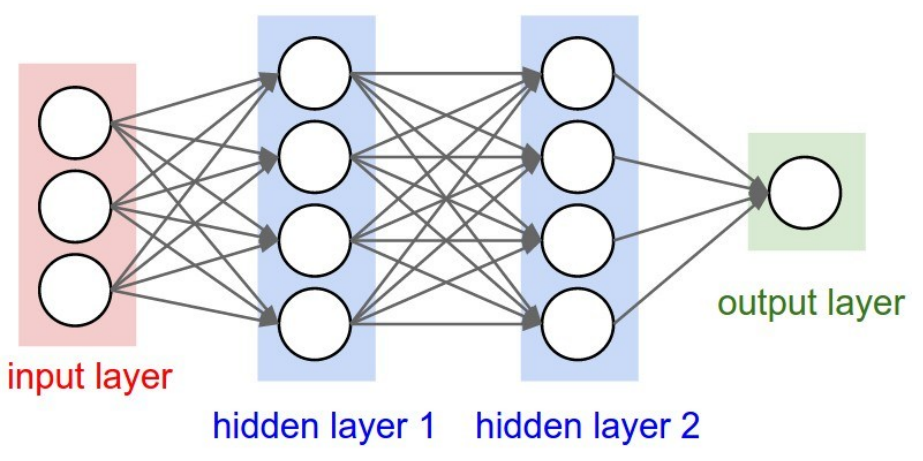
\includegraphics[width=.6\textwidth]{assets/vol-mlp-layers.png}
            \end{cimage}
        \item[CNN] $\rightarrow$ i livelli sono organizzati come griglie 3D di neuroni:
            \begin{cimage}
                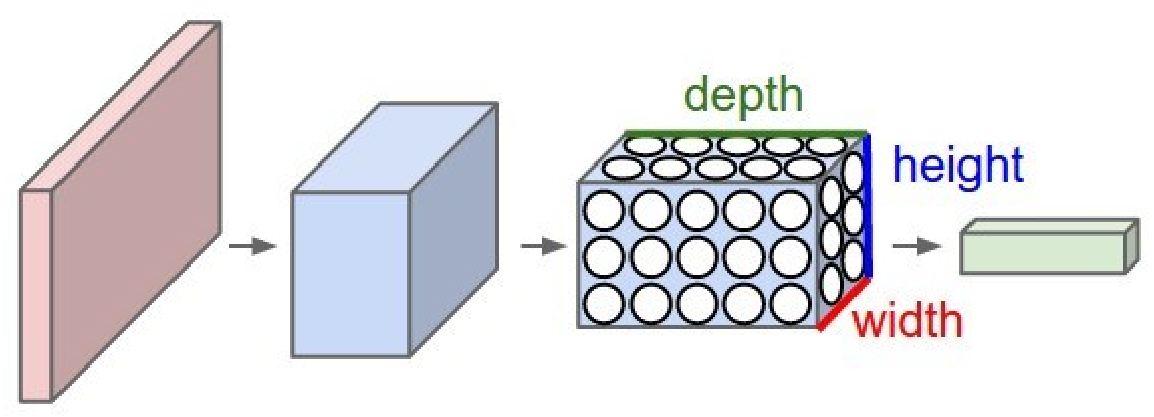
\includegraphics[width=.6\textwidth]{assets/vol-cnn-layers.png}
            \end{cimage}
            Sui piani \textbf{width - height} si conserva l'organizzazione spaziale <<retinotipica>> dell'immagine in input; mentre la terza dimensione \textbf{depth} individua le diverse \red{feature map}.
    \end{description}
\end{note}
%
% subsubsection Volumi (end)
% subsection Convoluzione (end)
%
\subsection{Convoluzione 3D}\label{sub:cnn_convoluzione_3d} % (fold)
Il filtro opera su una porzione del \textbf{volume} di input.
Nell'\hyperref[fig:cnn-conv-3d-es]{esempio} ogni neurone del volume di output è connesso a $5\times 5 \times 3 = 75$ neuroni del livello precedente.
\begin{cimage}
    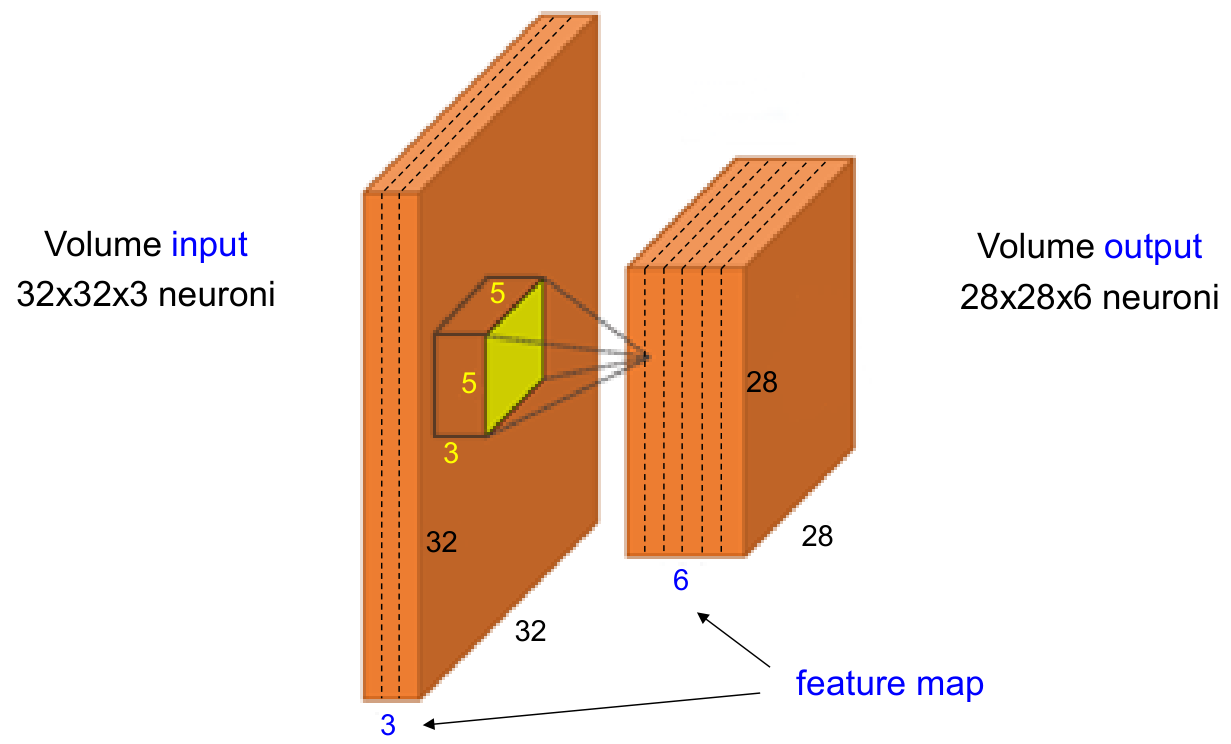
\includegraphics[width=.6\textwidth]{assets/cnn-conv-3d-es.png}
    \caption{}\label{fig:cnn-conv-3d-es}
\end{cimage}
Ciascuna fetta di neuroni (stessa \textbf{depth}) denota una \textbf{feature map}.
Nell'\hyperref[fig:cnn-conv-3d-es]{esempio} si trovano:
\begin{itemize}
    \item 3 feature map (dimensione $32\times32$) nel volume di input;
    \item 6 feature map (dimensione $28\times28$) nel volume di output;
\end{itemize}
I pesi sono \red{condivisi} a livello di \red{feature map}.
I neuroni di una stessa feature map processano porzioni diverse del volume di input nello stesso modo.
Ogni feature map può essere vista come il risultato di uno \textbf{specifico filtraggio} dell'input.
\begin{quote}
    Nell'esempio il numero di \red{connessioni} tra i due livelli è $\pt{28\times28\times6}\times\pt{5\times5\times3} = 352800$, ma il numero totale di pesi è $6 \times\pt{5\times5\times3 + 1} = 456$.
\end{quote}
Quando un filtro 3D viene fatto scorrere sul volume di input, invece di spostarsi con \textbf{passi} unitari si può utilizzare un passo, o \red{Stride} maggiore.
Questa operazione riduce la dimensione delle feature map nel volume di output e conseguentemente il numero di connessioni.
\begin{note}
    Sui livelli iniziali della rete per piccoli stride (2 o 4), è possibile ottenere un elevato guadagno in efficienza a discapito di una leggera penalizzazione in accuratezza.
\end{note}
Ulteriore possibilità, per regolare la dimensione delle feature map, è quella di aggiungere un \textbf{bordo} al volume di input.
Con il parametro \red{Padding} si denota lo spessore in pixel del bordo.
\emptyln{}
Sia $W_{out}$ la dimensione orizzontale della feature map di output e $W_{in}$ la corrispondente dimensione nell'input.
Sia inoltre $F$ la dimensione orizzontale del filtro.
Vale la seguente relazione:
\[
    W_{out} = \frac{\pt{W_{in} - F + 2 \cdot Padding}}{Stride} + 1
\]
% subsection Convoluzione 3D (end)
\subsection{Pooling}\label{sub:cnn_pooling} % (fold)
Un livello di \red{pooling} esegue un'\red{aggregazione} delle informazioni nel volume di input, generando feature map di dimensione \red{inferiore}.
L'obiettivo è quello di conferire \textbf{invarianza} rispetto a semplici trasformazioni dell'input mantenendo al tempo stesso le informazioni significative ai fini della discriminazione dei pattern.
\\
L'\red{aggregazione} opera nell'ambito di ciascuna feature map, cosicché il numero di feature map nel volume di input e di output è lo stesso.
Gli operatori di aggregazione più utilizzati sono la media ($Avg$) e il massimo ($Max$): entrambi <<piuttosto>> \red{invarianti per piccole traslazioni}.
Questo tipo di aggregazione \textbf{non ha parametri/pesi} da apprendere.
\begin{cimage}
    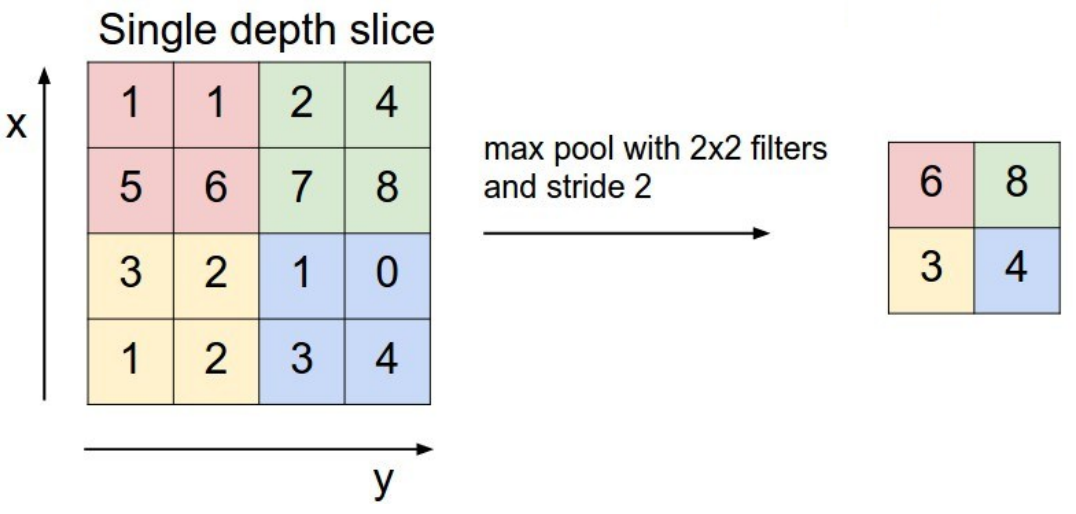
\includegraphics[width=.6\textwidth]{assets/cnn-pooling-visual.png}
\end{cimage}
% subsection Pooling (end)
\subsection{Training e Transfer Learning}\label{sub:cnn_training_e_transfer_learning} % (fold)
Il training di \ac{cnn} complesse su dataset di grandi dimensioni può richiedere giorni/settimane di tempo macchina anche se eseguito su GPU.
Fortunatamente, una colta che la rete è stata addestrata, il tempo richiesto per la classificazione di un nuovo pattern (\hyperref[sub:mlp_forward_propagation]{forward propagation}) è in genere \textbf{veloce}.
\\
Inoltre il training di una \ac{cnn} su un nuovo problema, richiede un \red{training set} etichettato di \textbf{notevoli dimensioni}.
In alternativa al training da zero, possiamo perseguire due strade (\textbf{Transfer Learning}):
\begin{itemize}
    \item \textbf{Fine-Tuning} $\rightarrow$ si parte con una rete \red{pre-trained} addestrata su un problema simile e:
        \begin{itemize}
            \item si \red{rimpiazza} il livello di output con un nuovo livello di output softmax (adeguando il numero di classi);
            \item come valori iniziali dei \red{pesi} si utilizzano quelli della rete pre-trained, tranne che per le connessioni tra il penultimo e ultimo livello i cui pesi sono inizializzati random;
            \item si eseguono nuove \red{iterazioni di addestramento} (\hyperref[sub:stochastic_gradient_descent]{SGD}) per ottimizzare i pesi rispetto alle peculiarità del nuovo dataset, non è necessario che sia di grandi dimensioni;
        \end{itemize}
        
    \item \textbf{Riutilizzo Features} $\rightarrow$ si utilizza una rete esistente, pre-trained, senza ulteriore fine-tuning.
        Si estraggono, a livelli intermedi, le feature generate dalla rete durante il passo forward.
        Si utilizzano queste feature per addestrare un classificatore esterno a classificare i pattern del nuovo dominio applicativo.
\end{itemize}
% subsection Training e Transfer Learning (end)
\begin{note}[Principali innovazioni nel deep learning]
    \begin{itemize}
        \item \textbf{Batch Normalization}, dopo ogni livello si normalizzano gli output affinché gli input al livello successivo non si spostino troppo nello spazio (\textbf{covariate shift}):
            \begin{quote}
                La normalizzazione avviene a livello di minibatch e di singola feature nelle \ac{cnn}.
                \\
                Il training è molto più stabile e veloce, con un learning rate maggiore.
            \end{quote}
        \item \textbf{Skip Connections}, si aggiungono dei collegamenti laterali ai layer che sommano l'input originario all'output del layer.
            In questo modo il mapping da apprendere è in termini di scostamento (o \red{residuale}) rispetto all'identità.
            Le reti sono più profonde e si riduce il problema di \hyperref[it:vani-grad]{vanishing gradient}.
    \end{itemize}
\end{note}
% section Convolutional Neural Network (end)
%
\section{Recurrent Neural Network}\label{sec:rnn} % (fold)
\subsection{Sequence to Sequence}\label{sub:rnn_sequence_to_sequence} % (fold)
Le reti \red{feedforward}, come \hyperref[sec:mlp]{MLP} o \hyperref[sec:cnn]{CNN}, studiate fino a questo momento, operano su \textbf{vettore di dimensione prefissata}.
\begin{cimage}
    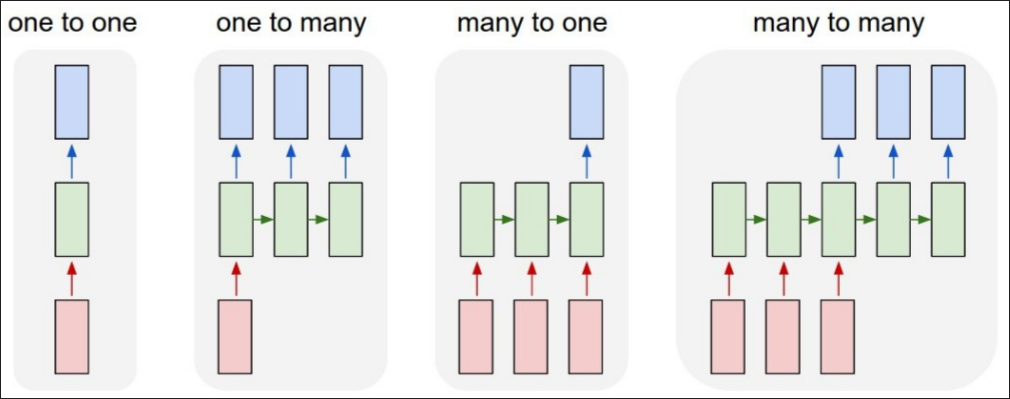
\includegraphics[width=.8\textwidth]{assets/seq-to-seq.png}
    \caption{}\label{fig:seq-to-seq}
\end{cimage}
Ad esempio l'input è un vettore immagine e l'output un vettore di probabilità delle classi.
Questo caso è rappresentato dalla prima colonna della \cref{fig:seq-to-seq} come sequenza \textbf{One to one}.
\\
\begin{quote}
    Applicazioni diverse richiedono che l'input e/o l'output possano essere sequenze, anche di lunghezza variabile.
\end{quote}
\begin{itemize}
    \item \textbf{One to many}, \red{image captioning} dove l'input è un'immagine e l'output è una frase (sequenza di parole) in linguaggio naturale che la descrive;
    \item \textbf{Many to one} \red{sentiment analysis} dove l'input è un testo e l'output un valore continuo che esprime il sentiment o giudizio (positivo o negativo);
    \item \textbf{Many to many} \red{language translation} dove l'input è una frase in Inglese e l'output la sua traduzione in italiano;
\end{itemize}
\begin{definition}{\acl{rnn}}{rnn}
    Le \textbf{reti ricorrenti} prevedono <<anche>> collegamenti all'indietro o verso lo stesso livello.
    I modelli più comuni e diffusi prevedono collegamenti verso \textbf{lo stesso livello}.
    \begin{cimage}
        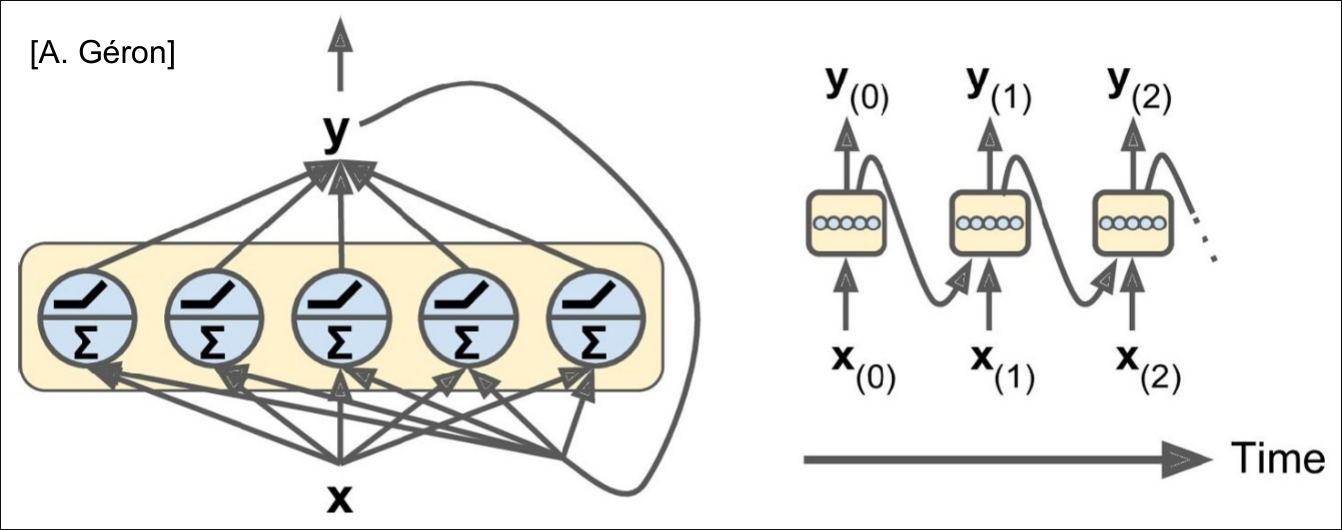
\includegraphics[width=.8\textwidth]{assets/rnn-time-visual.png}
    \end{cimage}
    A ogni step della sequenza, ad esempio a ogni istante temporale $t$, il livello riceve oltre all'\red{input} $x_\pt t$ anche il suo \textbf{output dello step precedente} $y_\pt{\dec t}$.
    Questo consente alla rete di basare le sue decisioni sulla \textbf{storia passata} ovvero su tutti gli elementi di una sequenza e sulla loro \textbf{posizione reciproca}.
\end{definition}
\begin{note}
    In una frase non è rilevante solo la presenza di specifiche parole ma è importante anche come le parole sono tra loro legate (posizione reciproca).
    \\
    La classificazione di video (sequenze di immagini) non necessariamente si basa sulle interrelazioni dei singoli frame.
\end{note}
% subsection Sequence to Sequence (end)
%
\subsection{Unfolding in Time}\label{sub:rnn_unfolding_in_time} % (fold)
Una \red{cell} è una parte di rete ricorrente che preserva uno \textbf{stato} interno $x_\pt t$ per ogni istante temporale.
È costituita da un numero prefissato di neuroni (può essere vista come layer).
\begin{note}
    $h_\pt t$ dipende dall'input $x_\pt t$ e dallo stato precedente:
    \[
        h_\pt t = \fx[h_\pt{\dec t},\, x_\pt t]
    \]
\end{note}
\begin{cimage}
    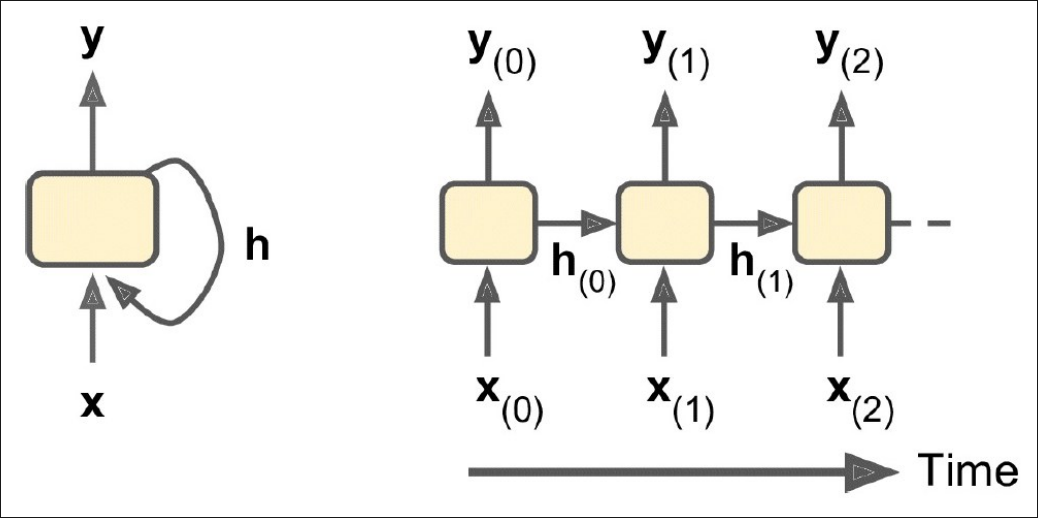
\includegraphics[width=.8\textwidth]{assets/unfold-time.png}
    \caption{}\label{fig:unfold-time}
\end{cimage}
Per poter addestrare, con \red{backpropagation}, una \ac{rnn} è necessario eseguire il cosiddetto \textbf{unfolding} o \textbf{unrolling in time} (parte destra della \cref{fig:unfold-time}), stabilendo a priori il numero d passi temporali su cui effettuare l'analisi.
\\
Di fatto una \ac{rnn} unfolded su 20 step equivale a una \ac{dnn} feedforward con 20 livelli.
Pertanto addestrare \ac{rnn} che appaiono relativamente semplici può essere molto costoso e critico per la convergenza (problema del \hyperref[it:vani-grad]{vanishing gradient}).
\begin{note}
    Da notare che in una \ac{rnn} unfolded: l'input e l'output sono in generale collegati a tutte le istanze della cella e i pesi della cella (nascosti in $f$) \textbf{sono comuni a tutte le istanze della cella}.
\end{note}
% subsection Unfolding in Time (end)
%
\subsection{Basic Cells, LSTM, GRU}\label{sub:rnn_basic_cells_lstm_gru} % (fold)
\subsubsection{Basic Cell}\label{sub:rnn_basic_cell} % (fold)
In una \red{cella base} di \ac{rnn}: lo stato $h_\pt t$ dipende dall'input $x_\pt t$ e dallo stato precedente $h_\pt{\dec t}$
\[
    h_\pt t = \phi\pt{x_{\pt t}^T \cdot W_x + h_\pt{\dec t}^T \cdot W_h + b}
\]
dove:
\begin{itemize}
    \item $W_x$ e $W_y$ sono i vettori dei pesi e $b$ il bias da apprendere;
    \item $\phi$ è la funzione di attivazione;
\end{itemize}
e l'output $y_\pt t$ corrisponde allo stato $h_\pt t$:
\[
    y_\pt t = h_\pt t
\]
Le celle base hanno difficoltà a ricordare/sfruttare input di step lontani: la memoria dei primi input \red{tende a svanire}.
D'altro canto sappiamo che in una frase anche le prime parole possono avere un'importanza molto rilevante.
\emptyln{}
Per risolvere questo problema e facilitare la convergenza in applicazioni complesse, sono state proposte celle più evolute dotate di un effetto \textbf{memoria a lungo termine}: \ac{lstm} e \ac{gru} sono le più note tipologie.
% subsubsection Basic Cell (end)
%
\subsubsection{LSTM}\label{sub:lstm} % (fold)
In \acl{lstm} lo stato $h_\pt t$ è suddiviso in due vettori $h_\pt t$ e $c_\pt t$:
\begin{itemize}
    \item $h_\pt t$ è uno stato, o memoria, a \textbf{breve termine}, anche in questo caso uguale all'output della cella $y_\pt t$;
    \item $c_\pt t$ è uno stato, o memoria, a \textbf{lungo termine};
\end{itemize}
La cella apprende durante il training cosa è importante \red{dimenticare} (\textbf{forget gate}) dello stato passato $c_\pt{\dec t}$ e cosa estrarre e aggiungere (\textbf{input gate}) dall'input corrente $x_\pt t$.
\begin{cimage}
    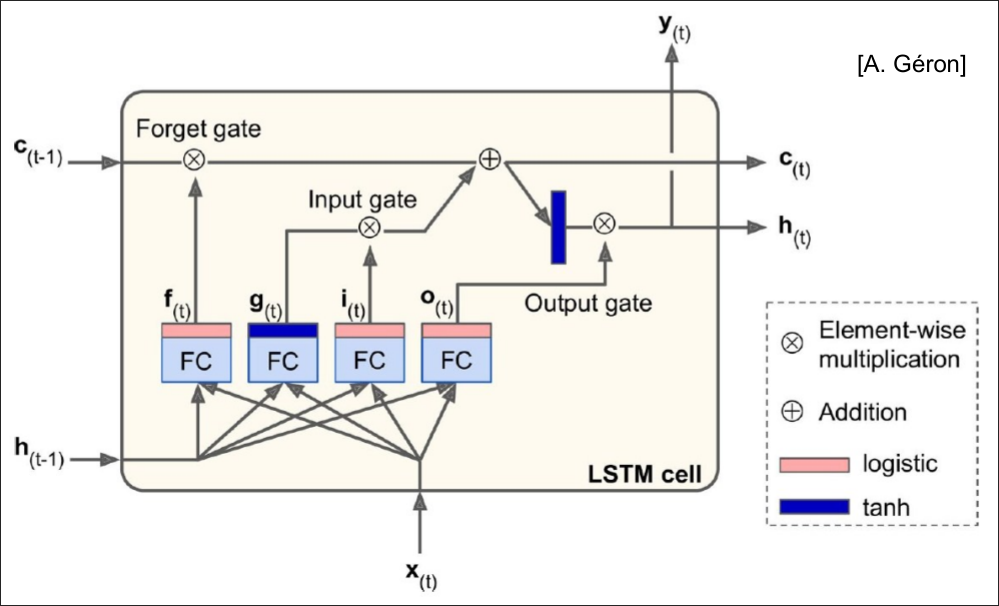
\includegraphics[width=.6\textwidth]{assets/lstm-visual.png}
\end{cimage}
Per il calcolo dell'output $y_\pt t = h\pt t$ si combina k'input corrente (\textbf{output gate}) con informazioni estratte dalla memoria a lungo termine.
% subsubsection LSTM (end)
%
\subsubsection{GRU}\label{sub:gru} % (fold)
\ac{gru} è una versione semplificata di \hyperref[sub:lstm]{LSTM}, che cerca di mantenere i vantaggi, riducendo i parametri e complessità.
\begin{cimage}
    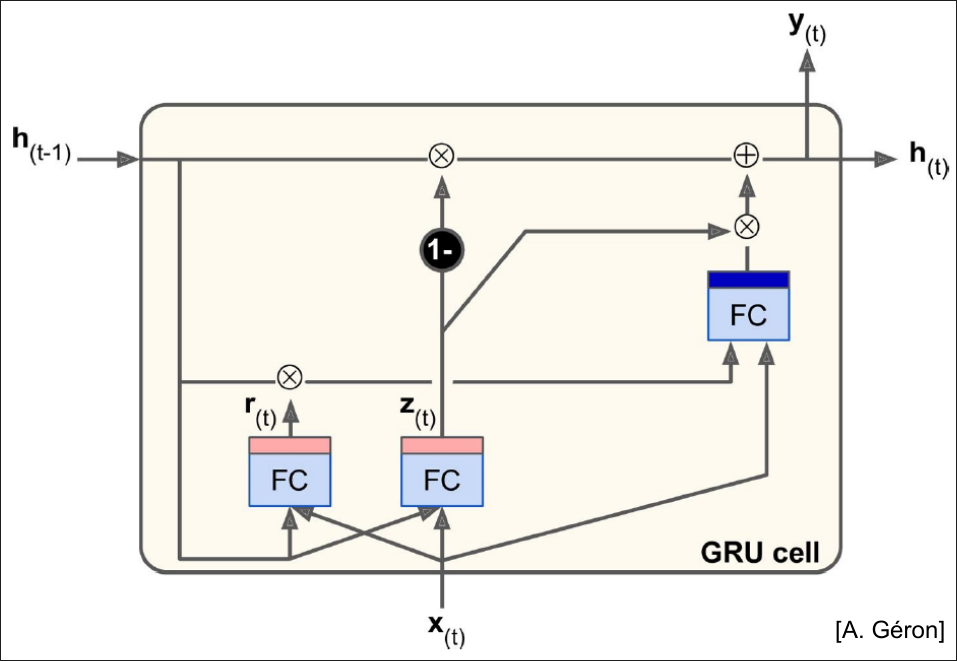
\includegraphics[width=.6\textwidth]{assets/gru-visual.png}
\end{cimage}
Le principali semplificazioni sono:
\begin{itemize}
    \item un solo stato di memoria $h_\pt t$;
    \item un solo gate, con logica invertita, per quantificare quanto dimenticare e quanto aggiungere: se necessario aggiungere prima di dimenticare;
\end{itemize}
% subsubsection GRU (end)
%
\subsubsection{Deep RNN}\label{sub:rnn_deep_rnn} % (fold)
\begin{cimage}
    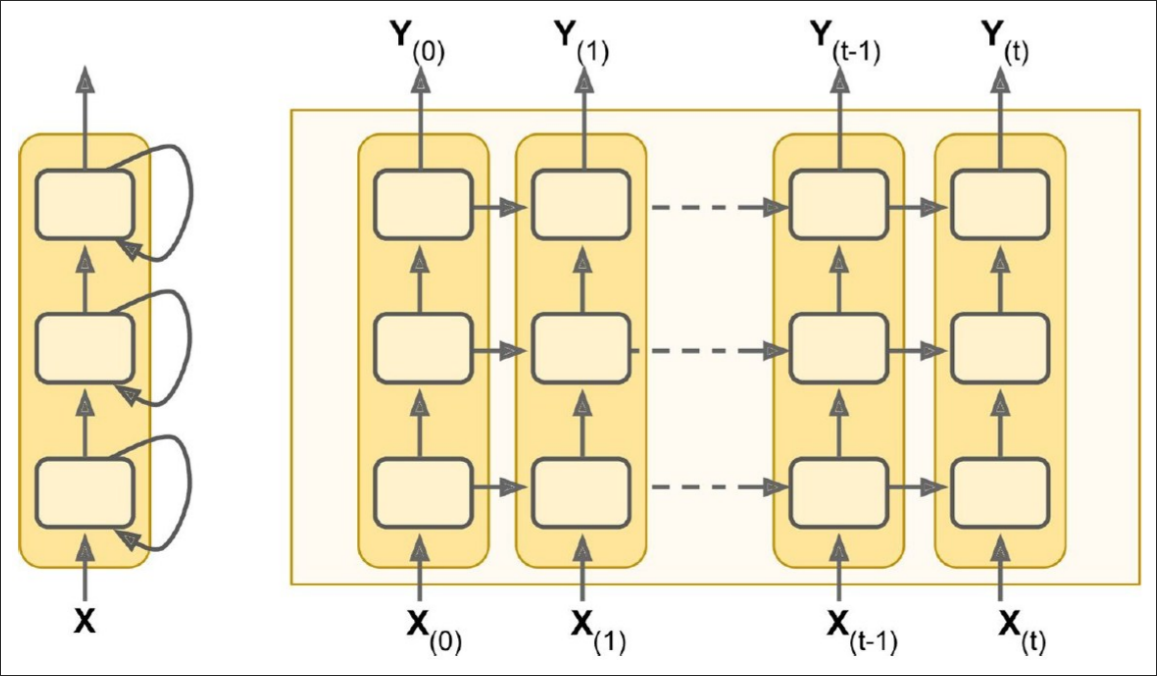
\includegraphics[width=.6\textwidth]{assets/deep-rnn.png}
    \caption{}\label{fig:deep-rnn}
\end{cimage}
In \cref{fig:deep-rnn} una \hyperref[def:rnn]{RNN} costituita da \red{tre layer} (stacked): a destra la versione unfolded (su $\inc t$ step):
\begin{itemize}
    \item gli output di un livello sono gli input del livello successivo;
    \item con più livelli possono essere apprese relazioni più complesse dei dati;
    \item l'addestramento supervisionato consiste sempre nel fornire gli input e gli output desiderati per il solo ultimo livello;
    \item se l'input sono immagini, i vettori $x_\pt t$ in genere non corrispondono ai pixel ma a feature di alto livello estratte da una \hyperref[sec:cnn]{CNN};
    \item se l'input sono parole, i vettori $x_\pt t$ sono il risultato di \textbf{word embedding};
\end{itemize}
% subsubsection Deep RNN (end)
% subsection Basic Cells, LSTM, GRU (end)
%
\subsection{Time Series, Dati statici e dinamici}\label{sub:rnn_time_series_dati_statici_e_dinamici} % (fold)
\begin{example}{}{}
    Una serie temporale (\textbf{time series}) può essere relativa all'andamento nel tempo: di un titolo di borsa, della temperatura di un ambiente, del consumo energetico di un impianto, ecc.
    \\
    Possiamo considerare una serie temporale come una funzione campionata in più istanti temporali.
    Conoscendo i valori fino all'istante $t$ siamo interessati a predire il valore a $\inc t$.
    \begin{cimage}
        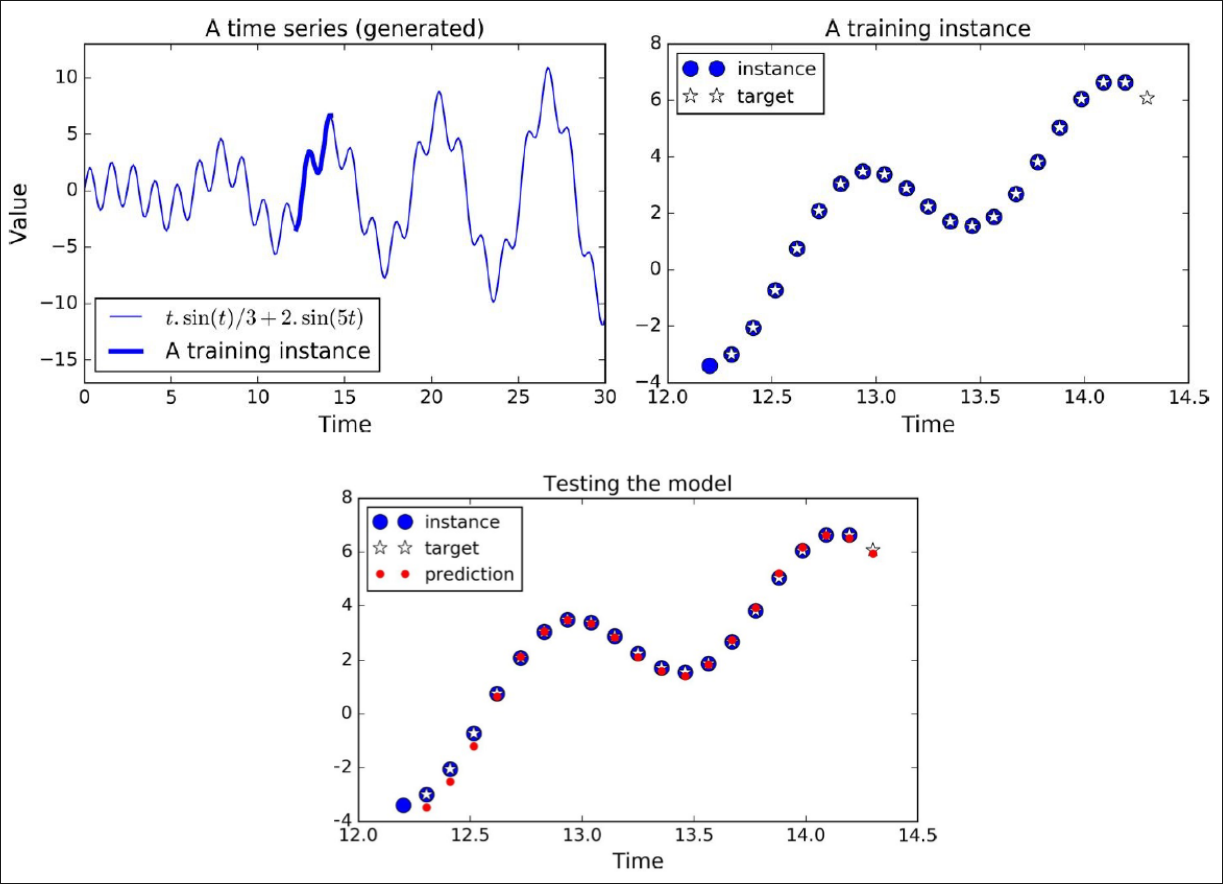
\includegraphics[width=.6\textwidth]{assets/time-series-ex-visual.png}
    \end{cimage}
\end{example}
Prima di proporre modelli complessi, con il serio rischio di overfitting, si provano semplici baseline, valutandone le prestazioni e la generalizzazione:
\begin{itemize}
    \item \textbf{persistence model}: la predizione al tempo $\inc t$ corrisponde al valore al tempo $t$;
    \item \textbf{linear model}: una semplice regressione lineare;
\end{itemize}
\begin{description}
    \item[Modelli statici classici] Le serie temporali sono state studiate per decenni in ambito statistico ed esistono molti metodi, relativamente semplici, e talvolta preferibili a reti ricorrenti:
        \begin{itemize}
            \item \textbf{decorrelazione} dei dati della sequenza: se i valori di una sequenza sono correlati nel tempo, si ha l'impressione di riuscire a predire con grande successo;
        \end{itemize}
\end{description}
%
\subsubsection{Classificazione/Regressione su Serie Temporali}\label{sub:rnn_classificazione_regressione_su_serie_temporali} % (fold)
\begin{cimage}
    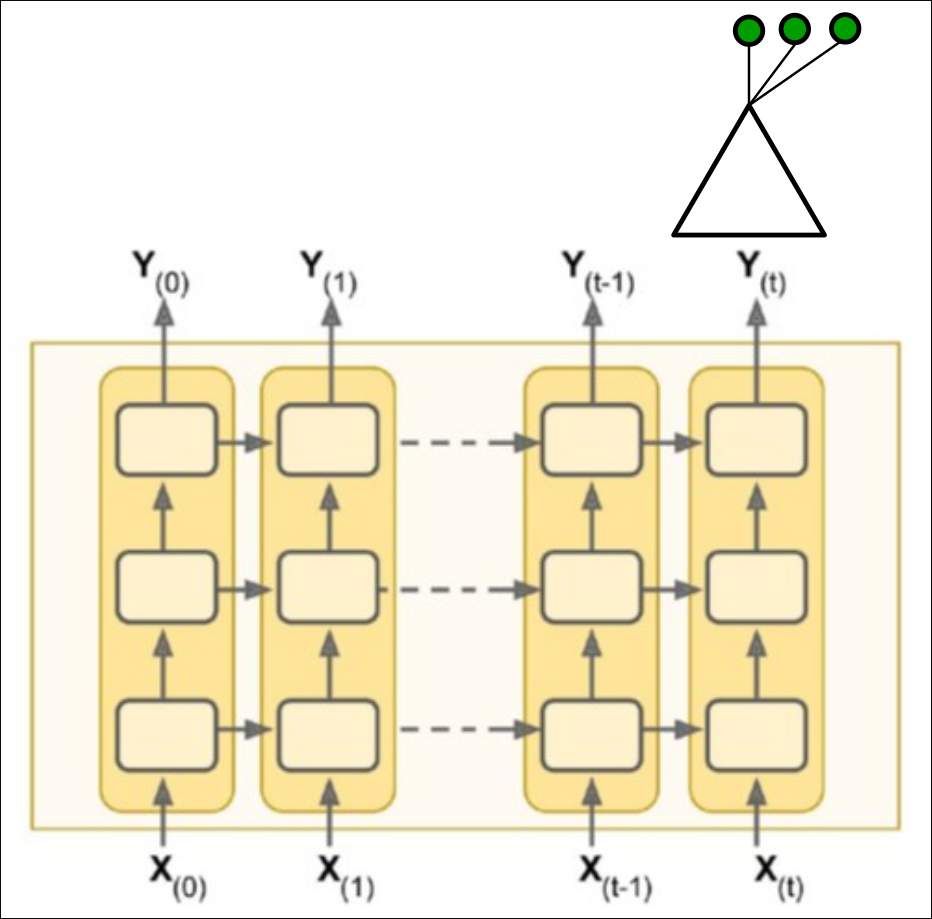
\includegraphics[width=.4\textwidth]{assets/class-regr-temp-ser-rnn.png}
\end{cimage}
Un semplice \hyperref[sec:mlp]{MLP} (con uno o pochi layer) è collegato al vettore $Y_\pt t$:
\begin{itemize}
    \item nel caso di classificazione, tanti neuroni di output quante sono le classi;
    \item nel caso di regressione, tanti neuroni quante sono le prediction ahead (uso tre neuroni per predire a $\inc t$, $t + 2$ e $t + 3$);
\end{itemize}
% subsubsection Classificazione/Regressione su Serie Temporali (end)
%
\subsubsection{Combinazione dati Statici e Dinamici}\label{sub:rnn_combinazione_dati_statici_e_dinamici} % (fold)
Talvolta solo un sottoinsieme dei dati disponibili varia nel time-frame considerato (dati \textbf{dinamici}).
Altri dati (\textbf{statici}) definiscono il contesto.
\begin{example}{}{}
    Informazioni di base di un paziente (\red{statici}) e l'evoluzione dei suoi livelli di glucosio (\red{dinamici}).
    Il sistema si modella:
    \begin{enumerate}
        \item si replicano i dati statici in tutte le osservazioni (da $X_\pt 0$ a $X_\pt t$) $\rightarrow$ poco efficiente;
        \item si forniscono i dati statici come input al \hyperref[sec:mlp]{MLP} finale $\rightarrow$ il modello ricorrente non è influenzato da essi (non ottimale);
        \item si utilizzano i dati statici per definire lo stato hidden $h$ di ingresso (non più inizializzato) $\rightarrow$ di fatto si crea un modello \textbf{encoder-decoder} dove l'encoder opera su un solo istante temporale (vettore dei dati statici) e produce lo stato iniziale (contesto) per il decoder;
    \end{enumerate}
    \begin{cimage}
        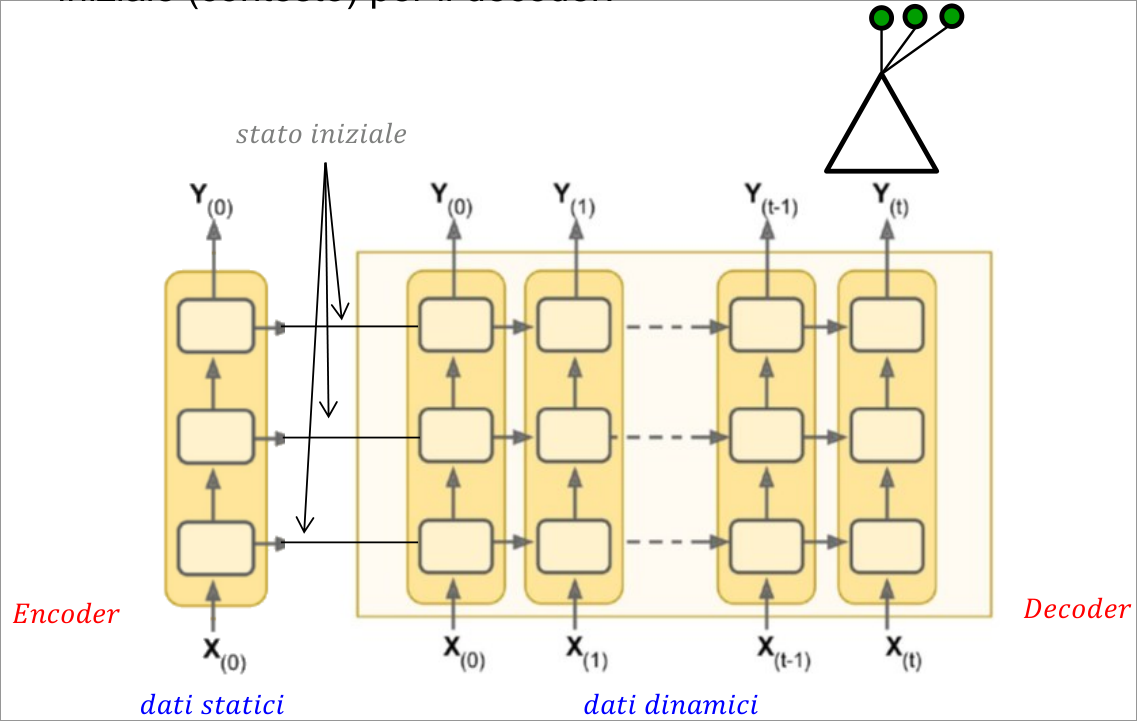
\includegraphics[width=.6\textwidth]{assets/rnn-data-static-dynamic.png}
    \end{cimage}
\end{example}
% subsubsection Combinazione dati Statici e Dinamici (end)
% subsection Time Series, Dati statici e dinamici (end)
% section Recurrent Neural Network (end)
%
\section{Natural Language Processing}\label{sec:nlp} % (fold)
L'elaborazione del linguaggio naturale è uno dei settori cui il deep learning ha dato i maggiori contributi.
Tra le principali applicazioni:
\begin{itemize}
    \item \textbf{Text Classification}: Sentiment Analysis;
    \item \textbf{Entity Extraction} (\textit{Named Entity Recognition}): estrarre dal testo non strutturato informazioni rilevanti;
    \item \textbf{Summarization}: generare riassunti concisi di documenti;
    \item \textbf{Generation}: generare testi in diversi ambiti specificando lo stile (applicazioni in ambito giornalistico/marketing);
    \item \textbf{Machine Translation}: traduzione tra lingue, ma anche tra linguaggi di programmazione;
    \item \textbf{Coding}: completamento intelligente del codice, creazione di funzioni da specifiche in linguaggio naturale, commenti automatici;
    \item \textbf{Question Answering}: rispondere in linguaggio naturale a domande poste in linguaggio naturale;
    \item \textbf{Digital Assistant e Chatbots}: dagli assistenti digitali a conversational AI;
    \item \textbf{Automatic Speech Recognition e Synthesis}: traduzione del parlato in testo e sintesi vocale;
    \item \textbf{Multimodal Extensions}: oltre al testo si utilizzano input/output di diversa natura (data un immagine generare una descrizione in linguaggio naturale);
\end{itemize}
%
\subsection{Tokenization - Embedding}\label{sub:nlp_token_embed} % (fold)

% subsection Tokenization - Embedding (end)
%
\subsection{Neural Machine Translation}\label{sub:nlp_neural_machine_translation} % (fold)

% subsection Neural Machine Translation (end)
%
\subsection{Transformers}\label{sub:nlp_transformers} % (fold)

% subsection Transformers (end)
%
\subsection{Large Language Models}\label{sub:nlp_large_language_models} % (fold)

% subsection Large Language Models (end)
%
\subsection{Prompt Engineering e Few-shot Learning}\label{sub:nlp_prompt_engineering_e_few_shot_learning} % (fold)

% subsection Prompt Engineering e Few-shot Learning (end)
%
\subsection{Embedding, Indexing, Tuning}\label{sub:nlp_embedding_indexing_tuning} % (fold)

% subsection Embedding, Indexing, Tuning (end)
% section Natural Language Processing (end)
%
\section{Reinforcement Learning}\label{sec:rl} % (fold)
\subsection{Q-Learning}\label{sub:rl_q_learning} % (fold)

% subsection Q-Learning (end)
%
\subsection{Deep Reinforcement Learning}\label{sub:rl_deep_reinforcement_learning} % (fold)

% subsection Deep Reinforcement Learning (end)
% section Reinforcement Learning (end)
% chapter Deep Learning (end)
